% Präambel
\documentclass[12pt,a4paper,oneside, 
liststotoc, 					% Tabellen- und Abbildungsverzeichnis ins Inhaltsverzeichnis
bibtotoc,						% Literaturverzeichnis ins Inhaltsverzeichnis aufnehmen
titlepage, 						% Titlepage-Umgebung statt \maketitle
headsepline, 					% horizontale Linie unter Kolumnentitel
%abstracton,					% Überschrift beim Abstract einschalten, Abstract muss dazu in {abstract}-Umgebung stehen
%DIV11,							% auskommentieren, um den Seitenspiegel zu vergrößern
BCOR6mm,						% Bindekorrektur, die den Seitenspiegel um 6mm nach rechts verschiebt,
]{scrreprt}			
\usepackage{ucs} 				% Dokument in utf8-Codierung schreiben und speichern
\usepackage[utf8x]{inputenc} 	% ermöglicht die direkte Eingabe von Umlauten
\usepackage[ngerman]{babel} 	% deutsche Trennungsregeln und Übersetzung der festcodierten Überschriften
\usepackage[T1]{fontenc} 		% Ausgabe aller zeichen in einer T1-Codierung (wichtig für die Ausgabe von Umlauten!)
\usepackage{graphicx}  			% Einbinden von Grafiken erlauben
\usepackage{amsmath}
\usepackage{amsfonts}
\usepackage{amssymb}
\usepackage{mathpazo} 			% Einstellung der verwendeten Schriftarten
\usepackage{textcomp} 			% zum Einsatz von Eurozeichen u. a. Symbolen
\usepackage{listings}			% Datstellung von Quellcode mit den Umgebungen {lstlisting}, \lstinline und \lstinputlisting
\usepackage{xcolor} 			% einfache Verwendung von Farben in nahezu allen Farbmodellen
\usepackage[intoc]{nomencl}  	% zur Erstellung des Abkürzungsberzeichnisses
\usepackage{fancyhdr}			% Zusatzpaket zur Gestaltung von Fuß und Kopfzeilen
\usepackage{titleref}			% Zum referenzieren mit Überschrift
\usepackage{varwidth}			%alighn asci figure
\usepackage{chngcntr}			% Tabellen- und Abbildungsverzeichnis als fortlaufende Nummer
\usepackage{hyperref}
\usepackage[justification=centering]{caption} % Bild unterschrift mittig ausrichten
\usepackage{nameref}
\counterwithout{figure}{chapter}
\counterwithout{table}{chapter}
\usepackage{url}


%For flow chart
\usepackage{tikz}
\usetikzlibrary{shapes,arrows}
% Define block styles
\tikzstyle{decision} = [diamond, draw, fill=blue!20, 
    text width=4.5em, text badly centered, node distance=3cm, inner sep=0pt]
\tikzstyle{block} = [rectangle, draw, fill=blue!20, 
    text width=5em, text centered, rounded corners, minimum height=4em, node distance=3cm]
\tikzstyle{line} = [draw, -latex']
\tikzstyle{cloud} = [draw, ellipse,fill=red!20, node distance=2cm,
    minimum height=2em]


%\usepackage[none]{hyphenat} %deaktiviert Silbentrennung
%\usepackage{showframe}% zum Anzeigen des Seitenlayouts
%Abstand vor Chapter
\renewcommand*\chapterheadstartvskip{\vspace*{-\topskip}}
\renewcommand*\chapterheadendvskip{%
  \vspace*{1\baselineskip plus .1\baselineskip minus .167\baselineskip}}


\setlength\abovedisplayshortskip{0pt}
\setlength\belowdisplayshortskip{0pt}
\setlength\abovedisplayskip{20pt}
\setlength\belowdisplayskip{20pt}

% -----------------------------------------------------------------------------------------------------------------
% Zum Aktualisieren des Abkürzungsverzeichnisses bitte auf der Kommandozeile folgenden Befehl aufrufen :
%  makeindex Bachelorarbeit.nlo -s nomencl.ist -o Bachelorarbeit.nls
% -----------------------------------------------------------------------------------------------------------------

% Hier die persönlichen Daten eingeben:

\newcommand{\titel}{DLRG Dienstplan}
\newcommand{\untertitel}{Benutzerhandbuch für das DLRG Dienstplan-Portal
 
\url{https://dlrgdienstplan.de/}}
\newcommand{\autor}{Philippe Käufer}

\newcommand{\ovretextfalt}{%
DLRG LV Württemberg e.V. \\
Bezirk Stuttgart \\
Mühlhäuser Str. 319 \\
70378 Stuttgart \\
www.DLRG-Stuttgart.de \\
}

% Abkürzungen
\newcommand{\ua}{\mbox{u.\,a.\ }}
\newcommand{\zB}{\mbox{z.B.\ }}
\newcommand{\bs}{$\backslash$}
\newcommand{\Csharp}{C\#}

\renewcommand{\nomname}{Abkürzungsverzeichnis}
\makenomenclature 

% -------------------------------------------------------------------------------------------
% Definition der Kopf- und Fußzeilen
\lhead{}								% Kopf links
\chead{}								% Kopf mitte
\rhead{\sffamily{\titel}}				% Kopf rechts
\lfoot{}								% Fuß links
\cfoot{\sffamily{\thepage}}				% Fuß mitte
\rfoot{\sffamily{\autor}}				% Fuß rechts
\renewcommand{\headrulewidth}{0.4pt}	% Liniendicke Kopf
\renewcommand{\footrulewidth}{0.4pt}	% Liniendicke Fuß

\makenomenclature						% Abkürzungsverzeichnis erstellen

% alle Abkürzungen, die in der Bachelorarbeit verwendet werden

\nomenclature{CI}{Corporate Identity }

\nomenclature{ORM}{Objektrelationale Abbildung (object-relational mapping) }

\nomenclature{GUI}{Grafische Benutzeroberfläche oder auch grafische Benutzerschnittstelle (graphical user interface) }

\nomenclature{RWD}{(Responsive Web Design) Die Größe und Auflösung der Displays auf Laptops, Desktop-PCs, Tablets und Smartphones können erheblich variieren. Aus diesem Grund ist das Erscheinungsbild und die Bedienung einer Website stark abhängig vom Endgerät. Aufgrund dessen werden Webseiten mit einem Design ausgestattet welches sich auf die unterschiedlichen Anforderungen der Endgeräte anpassen. \cite{Responsive_Webdesign}
}

\nomenclature{Dienst}{Eine Freiwilligenarbeit in der DLRG für eine definierte Zeit. Meist im Wasserrettungsdienst oder Freibad. Der Dienst definiert wann und eventuell wie lange und wo die Freiwilligearbeit zu tätigen ist. Ein Dienst enthält eine oder mehrere zu besetzende Positionen.}

\nomenclature{Position}{Eine zu besetzende Freiwillgearbeit mit vordefinierten vorraussetzungen wie Wissen und Können (Qualifikation). Eine Position ist immer einem Dienst zugeordnet.}

\nomenclature{Qualifikation}{Ein definiertes Wissen und Können welches meist durch Besuchen von Lehrgängen und Fortbildungen in der DLRG erlangt werden kann.}				% Datei mit Abkürzungen laden


% -------------------------------------------------------------------------------------------
%                     Beginn des Dokumenteninhalts
% -------------------------------------------------------------------------------------------
\begin{document}
\setcounter{secnumdepth}{2}					% Nummerierungstiefe fürs Inhaltsverzeichnis
\setcounter{tocdepth}{2}
\sffamily									% für die Titelei serifenlose Schrift verwenden

% ------------------------------ Titelei -----------------------------------------------------

\thispagestyle{plain}
\begin{titlepage}
\enlargethispage{4.0cm}
%\sffamily 								% Serifenlose Grundschrift für die Titelseite einstellen

\begin{tikzpicture}[remember picture,overlay]%
	\node (nw) at (current page.north west) {};
	\node [xshift=0.2\paperwidth] (ne) at (nw) {};
	\node (sw) at (current page.south west) {};
	\node [xshift=0.2\paperwidth] (se) at (sw) {};

	% Farbiges Feld links
	%\filldraw[fill=yellow!90!black, draw=yellow!90!black] (nw) rectangle (se);
	\node (bard) at (nw) [anchor=north west,fill=red,minimum width=0.2\paperwidth,minimum height=\paperheight] {};

	% DLRG Wortmarke
	\node [anchor=north west,yshift=-2.5cm] at (bard.north west) {%
		
\includegraphics[width=0.185\paperwidth]{Bilder/DLRG-GELB.png}%
	};
	
	
	% Textfeld TOP
	\node (ovretext) [anchor=north west,align=left,yshift=-2.5cm,xshift=12pt,font=\sffamily] at (bard.north east) {%
		\ovretextfalt%
	};

	% Grafik mitte
	\node [anchor=north west,yshift=-2cm] at (ovretext.center) {%
		
\includegraphics[height=8cm]{Bilder/DienstplanDLRG_Kalender.png}%
	};

	% Titel
	\node (titel) [anchor=north west,yshift=-7cm+-2cm,align=left,text width=0.6\paperwidth,font=\LARGE\sffamily] 
		at (ovretext.south west) {%
		\textbf{\titel}%
	};

	% Untertitel
	\node (undertitel) [anchor=north west,yshift=-6pt,align=left,text width=0.6\paperwidth,font=\large\sffamily] 
		at (titel.south west) {%
		\untertitel%
	};

	% Author
	\node (forfattare) [anchor=south west,yshift=4cm,xshift=12pt,align=left,font=\sffamily] 
		at (bard.south east) {%
		Authoren: \autor%
	};
	
	% Logo unten rechts
	\node (logo) [anchor=south east,xshift=-18pt,yshift=18pt] at (current page.south east) {%
		
\includegraphics[width=0.2\paperwidth]{Bilder/Logo-B-Schwarz.png}%
	};
\end{tikzpicture}

\end{titlepage}
\rmfamily 				% erzeugt die Titelseite
\pagenumbering{Roman}						% große, römische Seitenzahlen für Titelei
\chapter*{Abstract} %*-Variante sorgt dafür, das Abstract nicht im Inhaltsverzeichnis auftaucht

Das DLRG Dienstplan-Portal dient zur Vereinfachung der Planung von Diensten im Ehrenamt. Der Prozess des Ausschreibens zu besetzender Dienste, der Helfer-Meldung wie auch jährlichen Statistik werden mit diesem Portal abgebildet.

\vspace*{5mm} \noindent Ziel ist es den ehrenamtlichen Helferinnen und Helfern eine Übersicht des aktuellsten Standes der Diensteinteilung wie auch selber Einflussmöglichkeiten zu geben. Die Helfer können selbst  partizipieren und Dienstwünsche direkt einreichen. 

\vspace*{5mm} \noindent Das Benutzerhandbuch für das DLRG Dienstplan-Portal hat den Zweck, eine Übersicht der Funktionen aus Sicht eines Anwenders zu geben. In diesem Dokument sind die einzelnen Funktionen und Prozesse im Detail erläutert und mit Grafiken als auch Beispielen aus der Anwendung verdeutlicht.   				% Einbinden des Abstracts

\tableofcontents							% Erzeugen des Inhalsverzeichnisses
\printnomenclature[2.0cm]					% Erzeugen des Abkürzungsverzeichnisses
\listoffigures 								% Erzeugen des Abbildungsverzeichnisses 
\listoftables 								% Erzeugen des Tabellenverzeichnisses
\pagebreak


% --------------------------------------------------------------------------------------------
%                    Inhalt der Bachelorarbeit
%---------------------------------------------------------------------------------------------
\pagenumbering{arabic}						% arabische Seitenzahlen für den Hauptteil
\pagestyle{fancy}					
\rmfamily
\noindent

\chapter{Einführung}
\label{cha:Einleitung}


\section{Quellcode und Lizenz}
\label{sec:licens_code}
Dieses Projekt steht unter der MIT Lizenz.

\vspace*{5mm} \noindent Copyright (c) 2017 \autor

\vspace*{5mm} \noindent Hiermit wird unentgeltlich jeder Person, die eine Kopie der Software und der zugehörigen Dokumentationen (die \glqq Software \grqq) erhält, die Erlaubnis erteilt, sie uneingeschränkt zu nutzen, inklusive und ohne Ausnahme mit dem Recht, sie zu verwenden, zu kopieren, zu verändern, zusammenzufügen, zu veröffentlichen, zu verbreiten, zu unterlizenzieren und/oder zu verkaufen, und Personen, denen diese Software überlassen wird, diese Rechte zu verschaffen, unter den folgenden Bedingungen:

\noindent Der obige Urheberrechtsvermerk und dieser Erlaubnisvermerk sind in allen Kopien oder Teilkopien der Software beizulegen.

\vspace*{5mm} \noindent DIE SOFTWARE WIRD OHNE JEDE AUSDRÜCKLICHE ODER IMPLIZIERTE GARANTIE BEREITGESTELLT, EINSCHLIEßLICH DER GARANTIE ZUR BENUTZUNG FÜR DEN VORGESEHENEN ODER EINEM BESTIMMTEN ZWECK SOWIE JEGLICHER RECHTSVERLETZUNG, JEDOCH NICHT DARAUF BESCHRÄNKT. IN KEINEM FALL SIND DIE AUTOREN ODER COPYRIGHTINHABER FÜR JEGLICHEN SCHADEN ODER SONSTIGE ANSPRÜCHE HAFTBAR ZU MACHEN, OB INFOLGE DER ERFÜLLUNG EINES VERTRAGES, EINES DELIKTES ODER ANDERS IM ZUSAMMENHANG MIT DER SOFTWARE ODER SONSTIGER VERWENDUNG DER SOFTWARE ENTSTANDEN.

\chapter{Registrierung}
\label{cha:register}

Die Registrierung ist auf der Startseite links unten (Abbildung  \ref{fig:view_login} \textit{\nameref{fig:view_login}}) zu finden.

\vspace*{5mm} \noindent Alle Felder sind Pflichtangaben. Wenn die selbe E-Mail Adresse wie bei dem eigenen Facebook Account verwendet wird, ist später ein Facebook Direkt-Login möglich. Das Passwort wird in der Datenbank verschlüsselt abgelegt. Die Administratoren können das Passwort nicht einsehen.

\begin{figure}[h]
 \begin{addmargin}{-0.2\linewidth}
   \centering 
   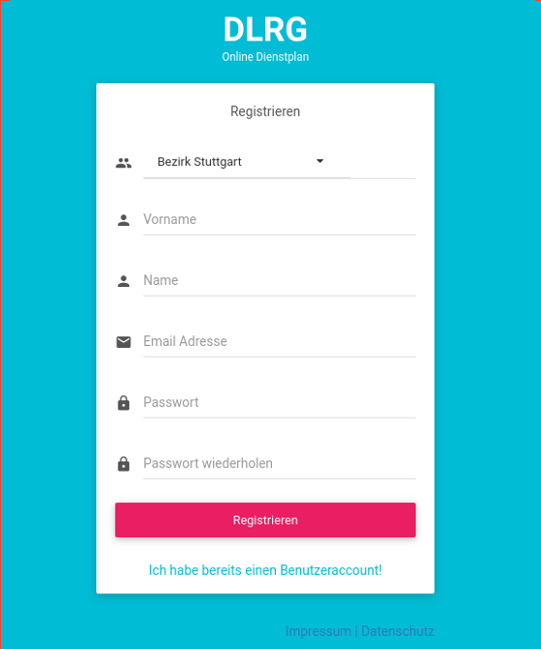
\includegraphics[width=10cm]{Bilder/view_register.png}
 \end{addmargin} 
 \caption[Registrierungs ansicht]{DLRG Dienstplan Registrierungs ansicht}
 \label{fig:view_register}
\end{figure}

\vspace*{5mm} \noindent 
Nachdem Registrungsvorgang muss der Account von einem Administrator freigeschaltet werden. Der Benutzer wird mit einer automatischen E-Mail benachrichtigt.

\noindent Nach dem erstmaligen Login sollte optional im Profil (siehe Kapitel \ref{sec:menu_profile} \textit{\nameref{sec:menu_profile}}) die Handynummer hinterlegt werden.
\chapter{Login}
\label{cha:login}

\begin{figure}[h]
 \begin{addmargin}{-0.2\linewidth}
   \centering 
   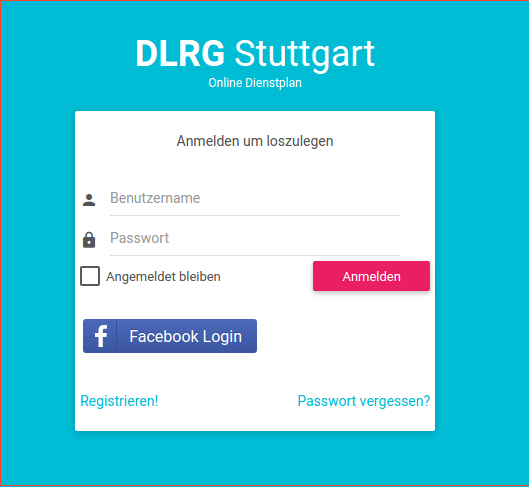
\includegraphics[width=10cm]{Bilder/view_login.png}
 \end{addmargin} 
 \caption[DLRG Dienstplan Login ansicht]{DLRG Dienstplan Login ansicht}
 \label{fig:view_login}
\end{figure}
\chapter{Menü}
\label{cha:menu}
\chapter{Qualifikationen}
\label{cha:qualification}
Ein Benutzer bekommt durch das Zuweisen von Qualifikationen die Rechte im Dienstplan eingetragen zu werden. Bei Zuweisung einer Qualifikation wir der Benutzer mit einer E-Mail benachrichtigt. Die Aktuell zugewiesenen Qualifikationen können über den Schnellzugriff (\ref{sec:menu_qualification} \textit{\nameref{sec:menu_qualification}}) eingesehen werden.

\noindent Qualifikationen sind ein zentraler Bestandteil um die Berechtigungen für Positionen zu erlangen. Positionen welche eine entsprechende Qualifikation voraussetzt, kann nur durch Benutzer mit dieser Qualifikation besetzt werden.

\noindent Bei neu erlangen von Qualifikationen (z.B. durch erfolgreichen Abschluss von Lehrgängen) müssen diese durch die Administratoren zugewiesen werden. Der Benutzer muss hier mit den Administratoren in Kontakt treten.

\vspace*{5mm} \noindent Sollte ein Benutzer zugriff auf mehrere Gliederungen haben, müssen die Qualifikationen von jeder Gliederung einzeln zugeteilt werden.
\chapter{Dashboard}
\label{cha:dashboard}

Das Dashboard bietet Überblicke und Statistiken:

\begin{itemize}
\item Geleistete Dienste: Summe der Dienste bei welchem der Benutzer eine Position übernommen hatte.
\item Total Geleistete Dienste: Summe der Positionen welche von allen geleistet wurde.
\item Noch nicht besetzte Dienste: Summe der zukünftig noch nicht besetzten Positionen. Hier werden nur Positionen welche für eine Mindestbesatzung relevant sind aufgezählt.
\item Hall of Fame: Benutzer mit den am meisten geleisteten Diensten. 
\end{itemize}

\noindent Darunter sind News (Kapitel \ref{cha:nachrichten}) wie auch neue Infos zu finden. Diese werden meist ebenfalls per E-Mail den Benutzern zugestellt.

\begin{figure}[h]
 \begin{addmargin}{-0.2\linewidth}
   \centering 
   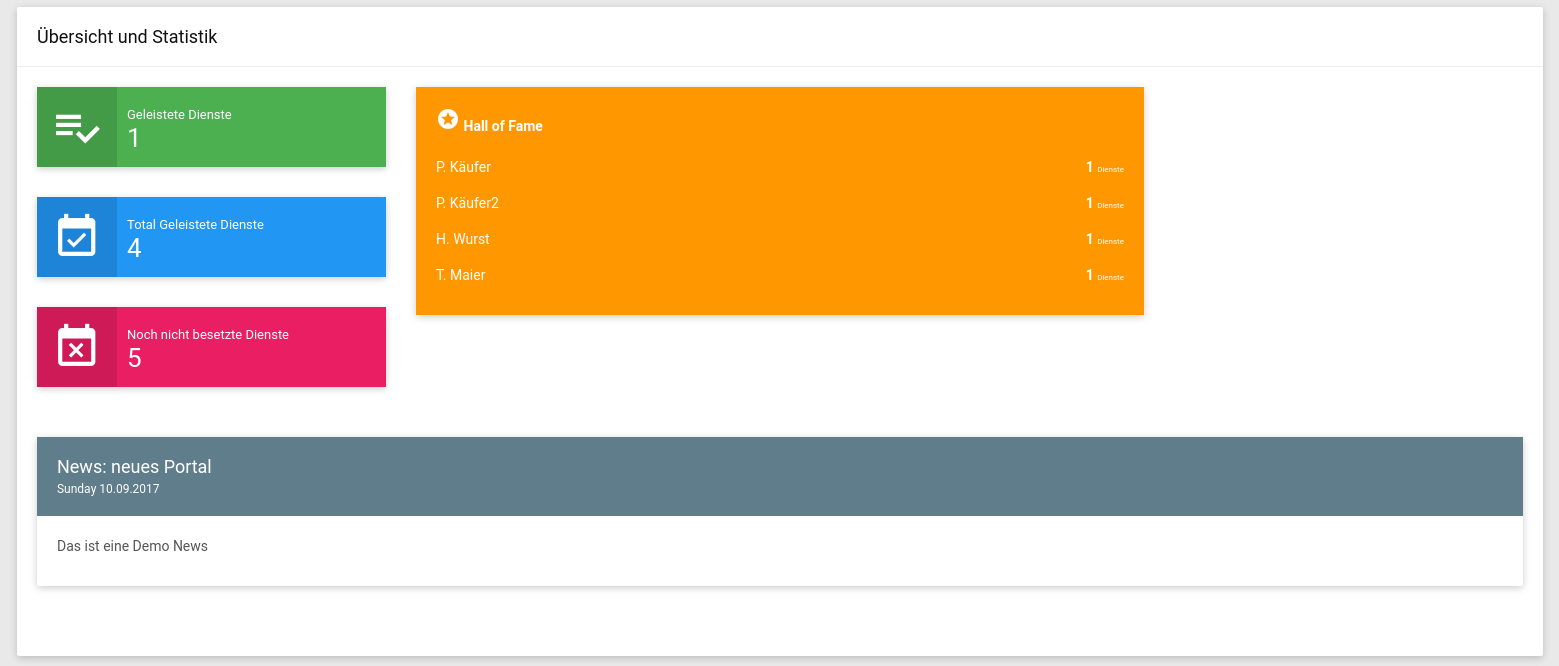
\includegraphics[width=20cm]{Bilder/view_overview.png}
 \end{addmargin} 
 \caption[Dashboard ansicht]{DLRG Dienstplan Dashboard ansicht}
 \label{fig:view_overview}
\end{figure}
\chapter{Dienste}
\label{cha:dienste}
Die Dienstübersicht zeigt alle zukünftigen Dienste absteigend sortiert nach Datum. Jeder Dienst wird als Block klar getrennt und übersichtlich dargestellt. In Abbildung \ref{fig:view_service} \textit{\nameref{fig:view_service}} ist ein einzelner Dienst exemplarisch abgebildet.

\begin{figure}[h]
 \begin{addmargin}{-0.2\linewidth}
   \centering 
   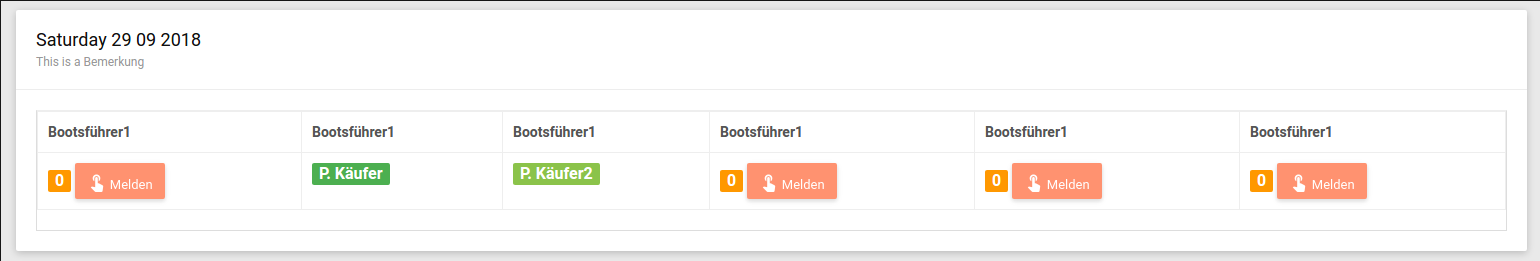
\includegraphics[width=20cm]{Bilder/view_service.png}
 \end{addmargin} 
 \caption[Dienste Übersicht]{DLRG Dienstplan Dienste Übersicht}
 \label{fig:view_service}
\end{figure}

\noindent Jeder Dienst ist mit Tag und Datum beschriftet. Darunter kann eine Bemerkung bzw. Beschreibung hinterlegt sein. Die einzelnen Positionen des Dienstes werden als Tabelle dargestellt.
\noindent Dem Benutzer kann eine Position in fünf verschiedenen Ansichten präsentiert werden mit welchen er zum teil Interagieren kann.
Diese sind in der folgenden Tabelle aufgezeigt. Beispiele beziehen sich immer auf die Abbildung \ref{fig:view_service} \textit{\nameref{fig:view_service}}

\begin{itemize}
\item Melden (bsp. Position 4): Diese Position ist noch nicht zugeteilt. Der Benutzer kann sich hierzu melden.
\item Melden deaktiviert (bsp. Position 1): Diese Position ist noch nicht zugeteilt. Der Benutzer hat aber nicht die entsprechende Qualifikation und kann sich somit für die Position nicht melden.
\item Position bestätigt (bsp. Position 2): Die Position ist bereits zugeteilt.
\item Position bestätigt (bsp. Position 3): Diese Position ist an den Benutzer zugeordnet. Alle zugeordneten Positionen des eigenen Benutzers werden zur besseren Übersicht hellgrün dargestellt.
\item Für Position gemeldet, noch nicht bestätigt (bsp. Position 5): Für diese Position hat der Benutzer sich bereits gemeldet. Solange dies durch die Administratoren noch nicht bestätigt ist, kann die Meldung zurück gezogen werden.
\end{itemize}

\noindent Die Zahl in den Orangenen Kästen vor dem Melde Button (bsp Position 4) gibt an, wie viele andere Benutzer sich bereits für diese Position gemeldet haben. Ein Benutzer kann sich für beliebig viele Positionen eines Dienstes melden. Ebenso können beliebig viele Benutzer sich für eine Position melden. Durch die Administratoren wird nur einer Benutzer für eine Position bestätigt.

\noindent Positionen können Kommentare beinhalten (bsp. Position 1). Mit Kommentaren können geteilte Positionen (Position 1 nur bis 14 Uhr) realisiert werden. Des weiteren können mit Kommentaren auch auf Besonderheiten zu dieser Position hingewiesen werden.


\section{Mobile Ansicht}
\label{sec:dienste_mobile}
Die GUI auf Mobilgeräten, wie \zB Smartphones oder Tablets, weicht von der Desktopversion leicht ab. Die einzelnen Dienste sind eingeklappt und können mit einem Tippen auf den kleinen Pfeil oder das Datum ausgeklappt werden (\ref{fig:view_service_mobile_close} \textit{\nameref{fig:view_service_mobile_close}}). 


\begin{figure}[h]
 \begin{addmargin}{-0.2\linewidth}
   \centering 
   
\includegraphics[width=20cm]{Bilder/view_service_mobile_close.png}
 \end{addmargin} 
 \caption[Dienste Übersicht Mobil]{DLRG Dienstplan Dienste Übersicht Mobil eingeklappt}
 \label{fig:view_service_mobile_close}
\end{figure}


\noindent Die rot hinterlegte Zahl zwischen dem kleinen Pfeil und dem Datum gibt die Anzahl der noch nicht zugewiesenen Positionen eines Dienstes an. In Abbildung \ref{fig:view_service_mobile} \textit{\nameref{fig:view_service_mobile}} ist die Zahl 6 dort zu sehen da wie in der ausgeklappten Ansicht zu sehen ist, 6 Positionen noch nicht zugewiesen wurden.

\begin{figure}[h]
 \begin{addmargin}{-0.2\linewidth}
   \centering 
   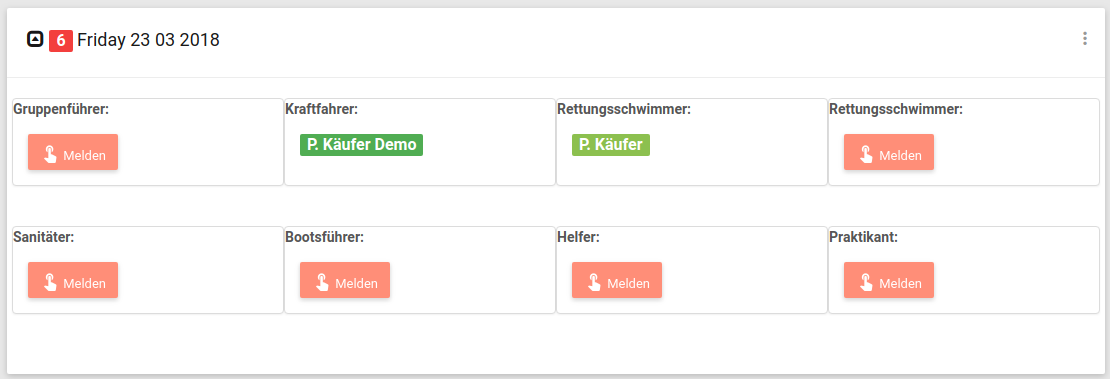
\includegraphics[width=20cm]{Bilder/view_service_mobile.png}
 \end{addmargin} 
 \caption[Dienste Übersicht Mobil Ausgeklappt]{DLRG Dienstplan Dienste Übersicht Mobil ausgeklappt}
 \label{fig:view_service_mobile}
\end{figure}
\chapter{Nachrichten}
\label{cha:nachrichten}
\chapter{Registrierung}
\label{cha:register}

\chapter{Login}
\label{cha:login}

\chapter{Menü}
\label{cha:menu}

\chapter{Qualifikationen}
\label{cha:qualification}

\chapter{Dienste}
\label{cha:dienste}

\chapter{Übersicht}
\label{cha:uebersicht}

\chapter{Nachrichten}
\label{cha:nachrichten}
\chapter{Aussicht}
\label{cha:aussicht}
Das DLRG Dienstplan-Portal soll stetig weiterentwickelt und verbessert werden. Hierzu sind im allgemeinen Feedback und Vorschläge immer willkommen!

\vspace*{5mm} \noindent Fehler, Erweiterungen und Wünsche werden bei der Codeverwaltung mit geführt: \url{https://github.com/Philhil/DienstplanDLRG/issues}
Direkte Einflussnahme und Diskussion zu Verbesserungen kann dort geschehen oder über E-Mail.

\vspace*{5mm} \noindent Funktionen die in Zukunft folgen:

\begin{itemize}
\item Mobile Ansicht: Die Mobile Ansicht für Smartphones soll optimiert werden.
\item Spezial Aufgaben: Es ist wünschenswert Spezialaufgaben wie z.B. Kochen für einen Dienst im DLRG Dienstplan-Portal festzulegen. 
\item Message Funktion innerhalb eines Dienstes: Für die vorab Kommunikation einer Dienst-Mannschaft ist es hilfreich dort eine direkte Kontaktmöglichkeit zu schaffen. Denkbar: Gruppenführer kann E-Mail versenden, Whatsapp Gruppe erstellen...
\item Kalender Funktion: Jeder Benutzer kann für sein Handy/Desktop Kalender den Dienstplan abbonieren. Bestätigte (und gemeldete?) Dienste würden so direkt im gewohnten Kalender vermerkt.
\item Hier könnte deine Idee stehen!
\end{itemize}
%


Für die Vorlage wird das paket \textit{listings} verwendet. \\

\begin{lstlisting} [language=PHP, numbers=left, numberstyle=\tiny, numbersep=10pt]
define('PATH_site', dirname(PATH_thisScript).'/');

if (@is_dir(PATH_site.'typo3/sysext/cms/tslib/')) {
        define('PATH_tslib', PATH_site.'typo3/sysext/cms/tslib/');
} elseif (@is_dir(PATH_site.'tslib/')) {
        define('PATH_tslib', PATH_site.'tslib/');
} else {
      
}
\end{lstlisting}

Quellcodedarstellung 

\begin{verbatim}
user@client:~> texdoc listings
\end{verbatim}

mehr über die Möglichkeiten des Pakets.

------------------------------------------------------\\
\textbf{Notitzen}

20-25 Seiten (Ohne Anhang, inhaltsverzeichniss etc)

Aufgabenstellung

\begin{itemize}
\item[•] Einordnung der Aufgabenstellung in übergeordnete Prozesse/Geschäftsziele
\item[-] Verknüpfung zu Vorlesungsinhalten
\item[-] Praktische Lösung
\item[-] Kritische, inhaltliche Reflexion von Theorie und Praxis
\end{itemize}


------------------------------------------------------\\
\textbf{Form}
Weißes 
Schreibmaschinenpapier  DIN  A  4  (Gewicht  ca.  70  g/qm),  nur  einseitig  beschrieben.  Format:  1,5 
-
zeilig, je Zeile ca. 70 Anschläge, Schriftgröße 12 Punkte
(z.B. bei Arial, b
ei
anderen Schriften ggf. anzupa
s-
sen)
. Randabstand mindestens 2,5 cm allseits.


------------------------------------------------------\\
\textbf{Gliederung der Arbeit}
Die Arbeiten sollten sich in folgende grobe Blöcke unterteilen

\begin{enumerate}
\item Vorspann (Titelblatt, evtl.  Sperrvermerk, Erklärung 
zur Eigenleistung 
[
siehe  2.7
], 
Zusammenfassung
in 
deutsch und englisch, Inhaltsverzeichnis, Abkürzungsverzeichnis, Abbildungs
-
und Tabellen
verzeichnis, 
evtl. Formelgrößen, evtl. Vorwort)

\item Einleitung  (Gegenstand  und  Ziele  der  Arbeit/Aufgabenbeschreibung,  Einführung  in  Thema,  Stand  der 
Technik/Forschung, Motivation der Aufgabenstellung/Vorausblick)
\item 
Hauptteil  (Anforderungsdefinition, 
Anforderungsanalyse,  Lösungsgenerierung,  Lösungsbewertung,  U
m-
setzung) in sinnvollen Gliederungspunkten
\item 
Zusammenfassung und Ausblick
\item 
Literaturverzeichnis
\item 
Anhänge

\end{enumerate}

------------------------------------------------------\\
\textbf{Gestaltung der inhaltlichen Abschnitte/Kapitel}

Einleitung
Die Einleitung soll den Ausgangspunkt der Arbeit umreißen, in kurzer Form zur Problemstellung hinführen 
und das Interesse des Lesers für die Arbeit wecken.
All
gemeine Einleitung ins Thema, keine Unternehmens
-
oder Produktbeschreibungen, Organigramme u.ä., wenn diese nicht direkt zum Thema führen.
Ziele und Vorgehensweise nicht vermischen.
Aufgabenstellung
Die Fragestellung der Aufgabe ist zu präzisieren. 
Insbesondere sind das Umfeld, die vorhandenen Randb
e-
dingungen und Betrachtungsgrenzen darzustellen.
Stand der Technik
Ausgehend von der Aufgabenstellung ist der derzeitige Stand der Technik für die Lösungsfindung zu b
e-
schreiben. Es sind z. B. die Vor
-
und 
Nachteile bisheriger Lösungen bzw. fundamentaler Lösungsprinzipien 
anhand der Literatur darzulegen.
Hauptteil
Der Text soll knapp und klar sein und die wesentlichen Gedanken der Arbeit beinhalten. Ein gewähltes Ve
r-
fahren oder ein bestimmter Lösungsweg muss
begründet werden. Es ist nicht notwendig, alle Vorversuche 
einzeln zu schildern. Bei Versuchen sind Voraussetzungen und Vernachlässigungen sowie die Anordnung, 
Leistungsfähigkeit und Messgenauigkeit der Versuchsanordnung anzugeben.
Die Ergebnisse der Arbe
it sind unter Berücksichtigung der Voraussetzungen ausführlich zu diskutieren und 
mit den bereits bekannten Anschauungen und Erfahrungen zu vergleichen.
Ziel der Arbeit ist es, eindeutige Folgerungen und Richtlinien für die Praxis zu finden.
Zusammenfassun
g 
Aufgabenstellung, Vorgehensweise und wesentliche Ergebnisse werden kurz und präzise dargestellt. 
Die 
Zusammenfassung ist eigenständig verständlich. Länge ca. 1 bis 1,5 Seiten.(Problem, Ziele, Vorgehenswe
i-
se, Ergebnisse und Ausblick).


% ---------------------------- Literaturverzeichnis ----------------------------------------------

\begin{thebibliography}{999999}

%\bibitem {Buchtitel} Author: \emph{Buchtitel}, Erscheinungsort: Verlag, Jahr

\bibitem {Responsive_Webdesign} Wikipedia: \emph{Responsive Webdesign}, \url{https://de.wikipedia.org/wiki/Responsive_Webdesign}, 15 12 2017.

\bibitem {Facebook_Login} Facebook: \emph{Facebook Login für das Web mit dem JavaScript-SDK}, \url{https://developers.facebook.com/docs/facebook-login/web}, 28 12 2017.


\end{thebibliography}

% ------------------------------- Anhang ---------------------------------------------------------

\begin{appendix}
\clearpage
\pagenumbering{Roman}						% römische Seitenzahlen für Anhang
\end{appendix}


\end{document}